\section{Einleitung}

Diese Arbeit befasst sich mit der Evaluation der Theorie, den Standards und Protokollen, ausgewählten Produkten, den Risiken und den Geschäftsmodellen, welche sich hinter dem Schlagwort \glqq Smart Home\grqq \ einreihen.
Ziel ist es, auch mit Hilfe der Methoden der Systemanalyse, mit falschen Vorstellungen aufzuräumen, den aktuellen Stand der Dinge darzulegen und einen Blick in die Zukunft der intelligenten Gebäude zu werfen.

\subsection{Definition: Smart Home}

Es existiert keine eindeutige Definition für Smart Homes.
Häufig wird unter Smart Home ein System verstanden, welches die Fähigkeit besitzt Beleuchtung, Temperatur, Zugang zum Gebäude und Unterhaltungsgeräte, wie z.B. ein Fernseher, über eine Schnittstelle zu kontrollieren.
Oft werden bei Smart Home Systemen auch alle Geräte mit einem zentralen sog. \glqq Hub\grqq \ verbunden, welcher die Nutzung verschiedener Komponenten auf Ressourcenschonung optimiert und automatisiert.
So werden Smart Home Systeme oft mit Energieeinsparungen beworben, welche sich daraus ergeben, dass z.B. nur geheizt wird, wenn auch Menschen anwesend sind.
Auch Komfortfunktionen, welche auf Automatisierungen, wie etwa dem automatischen Anschalten einer Zimmerlampe, wenn das Zimmer nicht mehr hell genug ausgeleuchtet ist und ein Mensch anwesend ist, werden oft zur Schau gestellt.\myfootcite[Vgl.][]{smart_home_def_usa,smart_home_def_cnbc}

Aschendorf erkennt in jedem Smart Home verallgemeinernd die Verbindung von Geräten, Automatisierungen und die Kontrolle über die verbundenen Geräte als elementare Bestandteile eines Smart Homes.\myfootcite[Vgl.][59ff]{aschendorf14}

Des Weiteren ist sogar der Begriff \glqq Smart Home\grqq \ nicht überall in Gebrauch. Im englischsprachigen Raum ist der Begriff \glqq Home automation\grqq \ (zu Deutsch \glqq Heimautomatisierung\grqq ) geläufig.
Auch \glqq Domotics\grqq \ (vom lateinischen Wort \glqq domus\grqq \ für \glqq Haus\grqq ) kann synonym genutzt werden.\myfootcite[Vgl.][]{smart_home_def_hill}

\subsection{Internet of Things}

Das \ac{IoT} hat zunächst nichts mit Heimautomatisierung zu tun.
Unter dem Internet der Dinge versteht man grundlegend die Verbindung von Geräten untereinander, sowie mit dem Internet.\myfootcite[Vgl.][]{ibm_iot}
Durch die Verbindung verschiedener Geräte, wie etwa einer Lichtschranke und einer Glühbirne, kann Mehrwert für den Benutzer der Geräte geschaffen werden, indem z.B. die Glühbirne automatisch bei Aktivierung der Lichtschranke aktiviert wird.
Zu einer Anwendung des \acp{IoT} wird das Beispiel, wenn das Internet noch mit involviert wird.
So wären hier Benachrichtigungen zu Bewegungsmeldungen oder Steuerung der Glühbirne über das Internet denkbar.

Ein Smart Home System kann also zum \ac{IoT}-System werden, wenn die Steuerung oder Automatisierung über eine Instanz im Internet abgewickelt wird.
Dies muss jedoch nicht der Fall sein.
So stellt die Software Home Assistant z.B. die Möglichkeit ein Smart Home System komplett offline zu betreiben.\myfootcite[Vgl.][]{hass_vision}

\section{Evaluation}

% TODO unter jede überschrift ein text...

\subsection{\textbf{TODO} Geschichte}

% idk -> wikipedia?

\subsection{Aufbau eines Smart Home Systems}

Aschendorf beschreibt den Aufbau von Smart Home Systemen als stufenförmige Hierarchie.
\autoref{fig:automatisierungspygramide} zeigt die drei Ebenen der Automatisierungspyramide nach Aschendorf:
Die Feldbusebene, die Automatisierungsebene und die Leitebene. \myfootcite[Vgl.][59]{aschendorf14}

\begin{figure}[ht]
	\centering
	\caption{Automatisierungspyramide nach Aschendorf}
	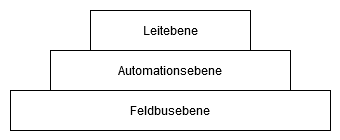
\includegraphics[scale=0.8]{Automatisierungspyramide_nach_Aschendorf}
	\caption*{\footnotesize{Quelle: Eigene Darstellung.}}
	\label{fig:automatisierungspygramide}
\end{figure}

\subsubsection{Feldbusebene}

Die Feldbusebene besteht aus sämtlichen eingebauten Systemkomponenten, also Gateways, welche verschiedene Systeme verbinden, Sensoren, welche z.B. Temperatur und Luftfeuchtigkeit überwachen, und Aktoren, wie z.B. Glühbirnen.
In der selben Ebene finden sich auch die Verbindungen der oben genannten Geräte wieder.
So ist die Feldbusebene in sich bereits funktional und direkt nutzbar.
Es kann z.B. der Sensor \textit{Lichtschalter 3} ausgelöst werden, welcher den Aktor \textit{Deckenlampe Wohnzimmer} aktiviert.\myfootcite[Vgl.][66-67]{aschendorf14}

\subsubsection{Automatisierungsebene}

Geräte übergreifende Automatisierungen werden in der Automatisierungsebene implementiert.
Dies wird durch einfache Controller oder programmierbare Mikrocomputer realisiert.
Nach der Änderung von Zuständen, wie z.B. der aktuellen Zeit, die Anwesenheit eines Bewohners oder die Temperatur eines Raumes, passt sich das Smart Home System mit dieser zusätzlichen Ebene nun nach vorgegebenen Regeln autonom an.\myfootcite[Vgl.][67-68]{aschendorf14}

\subsubsection{Leitebene}

Die Leitebene widmet sich der Interaktion des Smart Home Systems mit dessen Bewohnern.
Es lässt sich die Interaktion teilen in Eingaben und Ausgaben.
Zu den Eingaben zählen Befehle, die z.B. über Steuerungs-Apps gesendet werden oder von einem zentralen Steuerungscomputer emittiert werden.
Ausgaben werden etwa über digitale Dashboards auf diversen Displays angezeigt.
Über dieselben werden meist auch Fehlerdiagnosemeldungen angezeigt.\myfootcite[Vgl.][68-70]{aschendorf14}

% here we can use one of the required methods! (e.g. SSA)

\subsection{Verbindungssysteme}

In einem Smart Home System kommen Produkte verschiedener Art zum Einsatz.
Vom digitalen Kühlschrank, zum Türschloss hin zu Lichtschalter und Glühbirne.
Aufgrund der verschiedenenartigen Anwendungen der Produkte und den verschiedenen Herstellern werden im Smart Home Bereich verschiedene Verbindungssysteme und Protokolle verwendet.
Nachfolgend wird eine Auswahl der geläufigsten Systeme vorgestellt.

\subsubsection{LAN und WLAN}

2017 verfügten nach dem Statistischen Bundeamt 85,9\% aller deutschen Haushalte über einen stationären Internetzugang und damit einhergehend ein privates \ac{LAN} oder \ac{WLAN}.\myfootcite[Vgl.][]{haushalte}
Deshalb wird bei der nachträglichen Installation eines Smart Home Systems häufig auf \ac{LAN} oder \ac{WLAN} zurückgegriffen um Kosten und Installationsaufwand einzusparen.

Ein \ac{LAN} wird durch einen oder mehrere sog. Switches über Ethernet-Kabel verbunden.
Alternativ kann auch ein Router anstelle der Switches verwendet werden.
Dieser kann das \ac{LAN} sogar zusätzlich mit anderen \acp{LAN} verbinden, bspw. mit dem Internet.
Beim \ac{WLAN} wird an Stelle der Ethernet-Kabel über das 2,4 oder 5 GHz Band gefunkt.\myfootcite[Vgl.][]{local_area_network}

\begin{wrapfigure}{r}{0.35\textwidth}
	\centering
	\caption{Yeelight Glühbirne}
	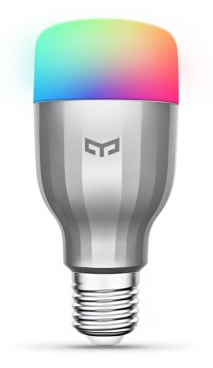
\includegraphics[scale=.5]{yeelight-bulb}
	\caption*{\footnotesize{Quelle: \mycite{figure_yeelight}}}
	\label{fig:yeelight}
\end{wrapfigure}

\autoref{fig:yeelight} zeigt die LED-Lampe \glqq Yeelight LED Bulb\grqq \ von Xiaomi, ein für Smart Home System Nachrüstungen gut geeignetes Produkt.
Die LED-Lampe nutzt das \ac{WLAN} zur Kommunikation mit der Steuerungskomponente und die vorhandene E27 Fassung zur Stromversorgung.\myfootcite[Vgl.][]{yeelight_wifi_bulb}

Der Einsatz von einem \ac{LAN} als Kommunikationssystem für Smart Home Anwendungen ist jedoch nicht uneingeschränkt zu empfehlen.
So sollte bedacht werden, dass die Integration eines beliebigen Smart Home Produkts Sicherheitslücken mit in das private \ac{LAN} reißen kann.
Bspw. könnte über das Ethernet-Kabel zu einer außen am Haus montierten Überwachungskamera auf das gesamte Heimnetzwerk zugegriffen und mitgelauscht werden.

\subsubsection{MQTT}

\ac{MQTT} ist ein speziell auf das \ac{IoT} ausgerichtetes Netzwerk-Protokoll.

\begin{figure}[ht]
	\centering
	\caption{MQTT Beispiel}
	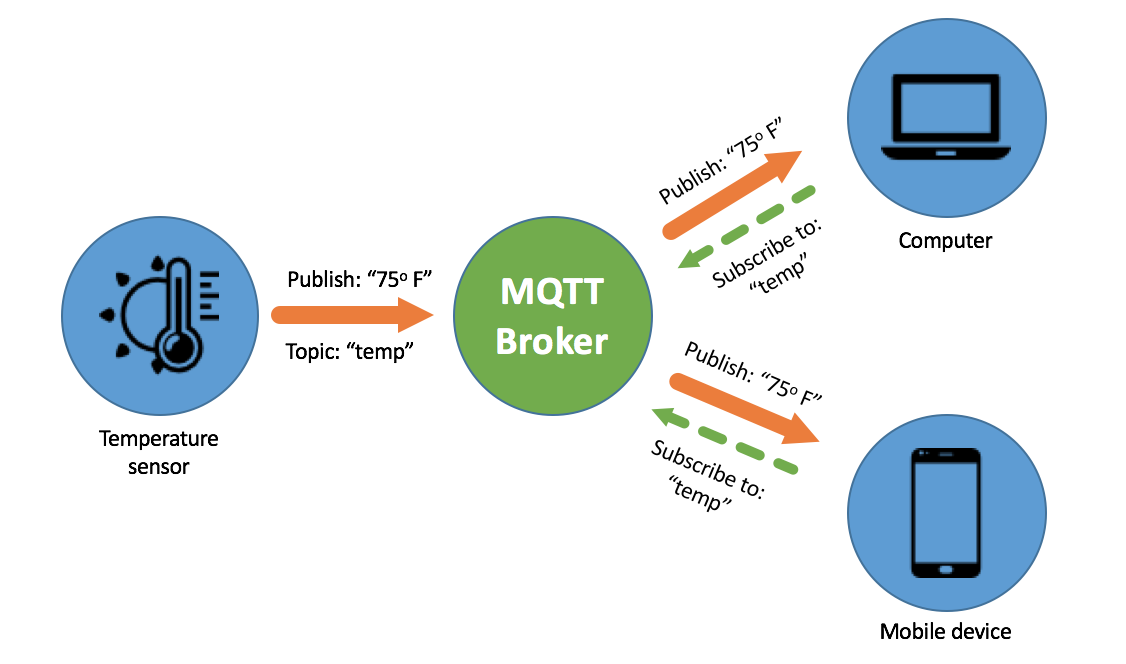
\includegraphics[scale=.4]{mqtt-example}
	\caption*{\footnotesize{Quelle: \mycite{figure_mqtt_architecture}}}
	\label{fig:mqtt_example}
\end{figure}

Anhand \autoref{fig:mqtt_example} lässt sich die Funktionsweise von \ac{MQTT} erklären.
Es gibt einen zentralen Server, den sog. Broker, über welchen diverse Geräte (die Clients) kommunizieren.
Dabei gibt es zwei Methoden:
Ein Client kann Daten zum Broker zu einem angegeben Thema senden und ein Client kann einem Broker mitteilen zu einem Thema informiert werden zu wollen.
Trifft eine Nachricht bei einem Broker ein schaut dieser nach, ob ihm zu dem entsprechenden Thema Abonennten bekannt sind und leitet ggf. die Nachricht weiter.
Kommunikation in \ac{MQTT} also nach dem Push-Prinzip statt, d.h. ein Client sendet keine Anfragen sondern erhält bei einem Ereignis eine Benachrichtigung.
Umgekehrt verfährt z.B. das \ac{HTTP}.
Zusätzlich garantiert \ac{MQTT} die Übermittlung einer Nachricht.
Bei Verbindungsabbruch oder Beschädigung der Nachricht wird die Nachricht weiter gesendet, bis das Senden erfolgreich verläuft.
Ebenso kann garantiert werden, dass eine Nachricht nur ein einziges Mal den Empfänger erreicht.\myfootcite[Vgl.][1]{mqtt_docs}

Anwendung findet das \ac{MQTT} Protokoll vorallem bei Sensoren für Raumtemperatur, Lichteinfall oder Bewegung, da hier eine lediglich eine eindimensionale Kommunikation abgebildet werden muss.
Da \ac{MQTT} ein offener und frei verfügbarer Standard ist, findet sich das Protokoll auch vermehrt in \ac{DIY}-Projekten wieder.\myfootcite[Vgl.][]{bruhautomation_esp_sensor}

Für die Nutzung von \ac{MQTT} spricht oft die Architektur des Protokolls, welche über den Broker das Senden von Nachrichten von vielen an viele ermöglicht.
Andererseits muss abgewägt werden, dass \ac{MQTT} auf Protokollebene keine Verschlüsselung nutzt.
Es können zwar auf höherer Ebene Sicherheitsfunktionen implementiert werden, jedoch würden diese die Geschwindigkeit des \ac{MQTT}-Protokolls signifikant verringern.\myfootcite[Vgl.][]{mqtt_pros_cons}

\subsubsection{ZigBee}

\begin{wrapfigure}{r}{0.4\textwidth}
	\centering
	\caption{ZigBee Stack}
	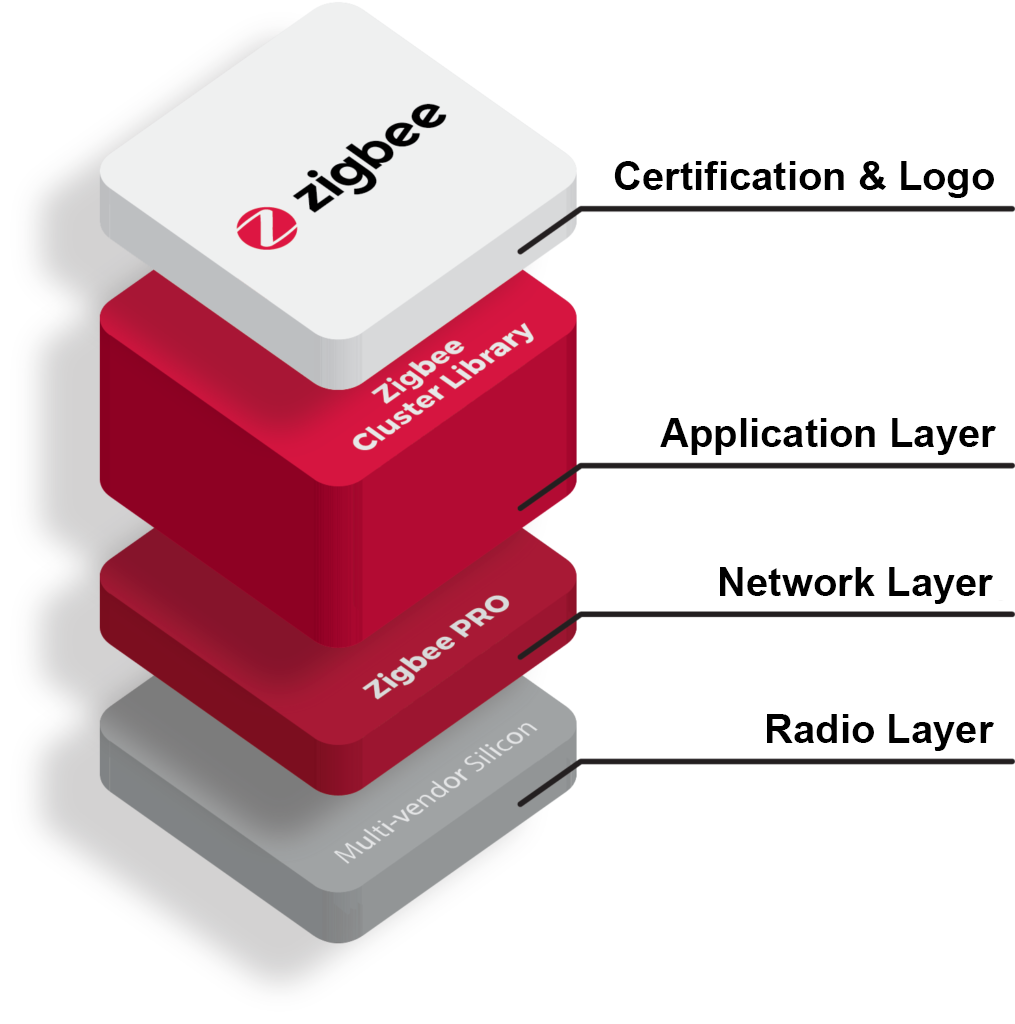
\includegraphics[width=0.4\textwidth]{zigbee-stack}
	\caption*{\footnotesize{Quelle: \mycite[Vgl.][]{figure_zigbee_stack}}}
	\label{fig:zigbee_stack}
\end{wrapfigure}

ZigBee ist eine Komplettlösung für das \ac{IoT}.
\autoref{fig:zigbee_stack} zeigt ZigBees Aufbau.
Die unterste Ebene stellt den Standard IEEE 802.15.4 dar - ein Übertragungsprotokoll für die untersten Ebenen eines \ac{WPAN}.
Auf dieser Ebene basiert die niedrigste Ebene ZigBees, die Netzwerkebene ZigBee PRO.
Diese ist global nutzbar, da das 2,4 GHz Band nach IEEE 802.15.4 definiert genutzt wird.
Die kennzeichnende Eigenschaft von ZigBee PRO ist jedoch die Vernetzung von Geräten, welche nicht nur schnell, sondern auch dezentral erfolgt.
So wird eine Nachricht etwa von einer Glühbirne, zu einer Steckdose, über einen Kühlschrank hin zu dem sog. ZigBee Hub gesendet, welches die Schnittstelle zur Interaktion mit ZigBee Geräten darstellt und somit die Reichweite und Signalstärke des ZigBee Netzwerkes erhöht.
Darüber hinaus implementiert ZigBee PRO Energiesparmechanismen, welche im Smart Home Sektor mit vielen Batterie betriebenen Geräten nützlich sind.
Ebenso liefert ZigBee PRO \ac{MQTT}-ähnliche Übertragungsarten, sowie eine Verschlüsselung der Kommunikation nach \ac{AES}.
Schließlich bietet die \ac{ZCL}, welche auf ZigBee PRO basiert, Entwicklern die Möglichkeit ZigBee einfach in eine beliebige Anwendung zu integrieren.
Die ZigBee-Zertifizierung eines Geräts stellt abschließend sicher, dass weitere Geräte nach ZigBee Spezifikation mit dem Gerät interagieren können.\myfootcite[Vgl.][]{zigbee_faq}

Der Beleuchtungssystemanbieter Signify nutzt ZigBee um Philips Hue Beleuchtungssyteme zuverlässig und kabellos zu installieren.
Gerade bei Gebäuden mit vielen massiven Wänden kann es von Vorteil sein ein \ac{P2P} System zu verwenden um ein Netzwerk aufzubauen, da zentrale Router nicht unbedingt alle Ecken eines Gebäudes abdecken können.\myfootcite[Vgl.][]{how_hue_works}

Für die Nutzung von ZigBee spricht vor allem die Interoperabilität zwischen verschiedenen ZigBee Geräten, welche durch die Zertifizierung und das global nutzbare 2,4GHz Band sichergestellt werden.
Damit werden ZigBee Systeme nicht nur einfach zu programmieren, sondern für Konsumenten auch einfacher zu installieren.
Die Möglichkeit \ac{P2P}-Netzwerke mit ZigBee Geräten zu bilden sorgt zudem für eine bessere Verbindung der einzelnen Geräte.
Schließlich können zusätzlich Batterie betriebene Geräte von ZigBees geringem Stromverbrauch profitieren.\myfootcite[Vgl.][]{zigbee_faq}

Es ist jedoch keine uneingeschränkte Empfehlung für ZigBee auszusprechen.
ZigBee ist zwar ein offener Standard, jedoch nicht kompatibel mit u.a. der \ac{GPL}.
Dies hat zur Folge, dass ZigBee nicht in freie Software implementiert werden kann.\myfootcite[Vgl.][]{iot_standard_war}
Außerdem besteht die Hürde eines jährlich zu entrichtenden Mitgliedsbeitrags um Zugang zu den ZigBee Spezifikationen und Standards zu erhalten, was Hobby-Programmierer und Bastler fern von ZigBee hält.\myfootcite[Vgl.][]{zigbee_membership}
Des Weiteren können herkömmliche Smartphones und Tablets nicht mit in ein ZigBee Netzwerk integriert werden, da diese nicht über den benötigten ZigBee Stack verfügen.
So muss immer ein ZigBee Hub installiert werden, welches die Schnittstelle zu herkömmlichen Systemen wie \ac{LAN} und \ac{WLAN} bildet.
Abschließend bleibt anzumerken, dass aufgrund der \ac{P2P}-Architektur ZigBees maximal Datenübertragungsraten von bis zu 250 kbit/s erreicht werden.\myfootcite[Vgl.][]{zigbee_faq}

\subsubsection{Z-Wave}

Z-Wave lässt sich nahezu identisch wie ZigBee beschreiben.\myfootcite[Vgl.][]{zwave_faq}
So wird auch eine \ac{P2P} Mesh Netzwerk-Topologie genutzt.

\begin{figure}[ht]
	\centering
	\caption{Star- vs. Mesh-Netzwerk}
	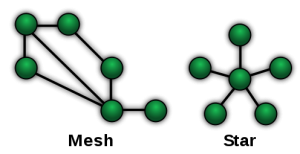
\includegraphics[scale=0.9]{star-vs-mesh-network}
	\caption*{\footnotesize{Quelle: \mycite{figure_star_vs_mesh_network}}}
	\label{fig:star_vs_mesh_network}
\end{figure}

\autoref{fig:star_vs_mesh_network} vergleicht die \ac{P2P} Mesh-Topologie mit der klassischen Stern-Topologie, wie sie z.B. bei einem \ac{WLAN} zu finden ist.
Bei einer Stern-Topologie sind alle Geräte im Netzwerk mit einem zentralen sog. Router verbunden, welcher die Nachrichten der Geräte einander entsprechend weiterleitet.
Bei einer Mesh-Topologie hingegen verbinden sich die Geräte mit allen Geräten in ihrer Reichweite.
Eine Nachricht an ein bestimmtes Gerät wird nun von Gerät zu Gerät geschickt, bis das empfangende Geräte das Empfänger-Gerät ist.
Hier müssen jedoch im Vergleich zur Stern-Topologie Abstriche bzgl. der Latzenz einer Nachricht gemacht werden, da eine Nachricht selten über eine direkte Verbindung gesendet werden kann.
Andererseits kann ein Mesh-Netzwerk einfacher expandiert werden, da jedes Gerät im Netzwerk Teil des Netzwerks ist.

Auch was den Energiebedarf eines Z-Wave Netzwerks anbelangt, kann kein Unterschied zu ZigBee festgestellt werden.
Beide Systeme ermöglichen es Batterie betriebenen Geräten über mehrere Jahre Nachrichten zu senden und zu empfangen, ohne Batterie-Wechsel.\myfootcite[Vgl.][]{smartcave_zwave_vs_zigbee}

\begin{wrapfigure}{r}{0.35\textwidth}
	\centering
	\caption{Z-Wave Chip}
	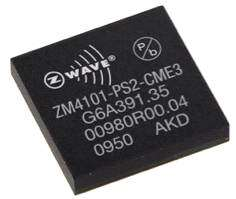
\includegraphics[width=0.35\textwidth]{zwave-chip}
	\caption*{\footnotesize{Quelle: \mycite{figure_zwave_chip}}}
	\label{fig:zwave_chip}
\end{wrapfigure}

Im Gegensatz zu ZigBee ist Z-Wave kein offener Standard.
So wird beim Bau eines Z-Wave kompatiblen Geräts ein proprietäres Bauteil benötigt.
\autoref{fig:zwave_chip} zeigt einen Z-Wave Funksendeempfänger von Sigma Designs aus 2012.
Dass die Hersteller von Z-Wave Geräten den Z-Wave Funksendeempfänger fremdbeziehen müssen bedeutet auf der einen Seite, dass Fehler im Z-Wave Funksendeempfänger nicht vom Hersteller korrigiert werden können und so evtl. Geräte zurückgerufen werden müssen, andererseits wird so sichergestellt, dass kein Hersteller das Herz eines jeden Z-Wave Geräts, die Kommunikationseinheit, verändert und somit die Interoperabilität aller Z-Wave Geräte nicht gefährden kann.\myfootcite[Vgl.][]{zwave_develop_a_product}

\begin{table}[ht]
	\caption{Z-Wave und ZigBee im Vergleich}
	\centering
	\begin{tabular}{| p{0.4\textwidth} | p{0.3\textwidth} | p{0.2\textwidth} |}
		\hline
		\textbf{Merkmal} 	& \textbf{Z-Wave} & \textbf{ZigBee} \\ \hline
		Kompatible Geräte & 2400+ & 2500+ \\ \hline
		Beteiligte Firmen & 418 & 322 \\ \hline
		Anzahl verkaufter Produkte & 100+ Mio.& 300+ Mio.\\ \hline
		Netzwerk-Topologie & Mesh & Mesh \\ \hline
		Max. Anzahl an Geräten im Mesh & 232 & ca. 65000 \\ \hline
		Genutzte Frequenzen & u.a. 868,4 MHz (EU); 908,4 MHz (US) & 2,4 GHz \\ \hline
	\end{tabular}
	\caption*{\footnotesize{Quellen: \mycite[Vgl.][]{zwave_product_count,zigbee_faq,zwave_member_count,safewise_zwave_vs_zigbee,zwave_faq,smartcave_zwave_vs_zigbee,zwave_frequencies,zigbee_member_count,zwave_products_sold}}}
	\label{tab:zwave_vs_zigbee}
\end{table}

Noch kann nicht abgeschätzt werden, ob sich Z-Wave oder ZigBee oder ein dritter \ac{IoT}-Standard durchsetzen wird.
Nach \autoref{tab:zwave_vs_zigbee} sind Z-Wave und ZigBee was beteiligte Firmen, kompatible Geräte und verkaufter Produkte angeht nahezu gleichauf.
Auf technischer Ebene sind die Standards zwar ähnlich, nicht aber gleich.
So kann mit ZigBee bspw. ein größeres Mesh-Netzwerk erstellt werden.
Hauptsächlich relevant beim Z-Wave-ZigBee-Vergleich sind jedoch die genutzten Frequenzen.
Da ZigBee das 2,4 GHz Band mit anderen Technologien wie z.B. \ac{WLAN} teilt, muss ZigBee mit Interferenzen operieren, während Z-Wave weitestgehend ungestört operieren kann.
Außerdem kann Z-Wave durch die geringere Frequenzen eine höhere Signalreichweite erzielen.
ZigBee hingegen erreicht durch die höhere Frequenz eine höhere Bandbreite.
Schließlich kann ZigBee auch wegen der globalen Nutzung der 2,4 GHz Frequenz regional limitiert kompatible Produkte vermeiden.
Z-Wave hingegen nicht.\myfootcite[Vgl.][]{zwave_faq}

\subsection{Amazon Alexa}

Amazon Alexa ist die Software für einen intelligenten Sprachassistenten, bestehend aus einem Lautsprecher, einem Mikrofon sowie einer Internetanbindung, welche seit 2014 in Alexa Geräten, wie in \autoref{fig:alexa_devices}, verbaut wird.\myfootcite[Vgl.][]{alexa_release}
Über die Internetanbindung wird auf ein Amazon Rechenzentrum zugegriffen, in welchem Ressourcen für die Verarbeitung von Spracheingaben mit \ac{ASR} und \ac{NLU} bereitgestellt werden.

\begin{figure}[ht]
	\centering
	\caption{Alexa Geräte}
	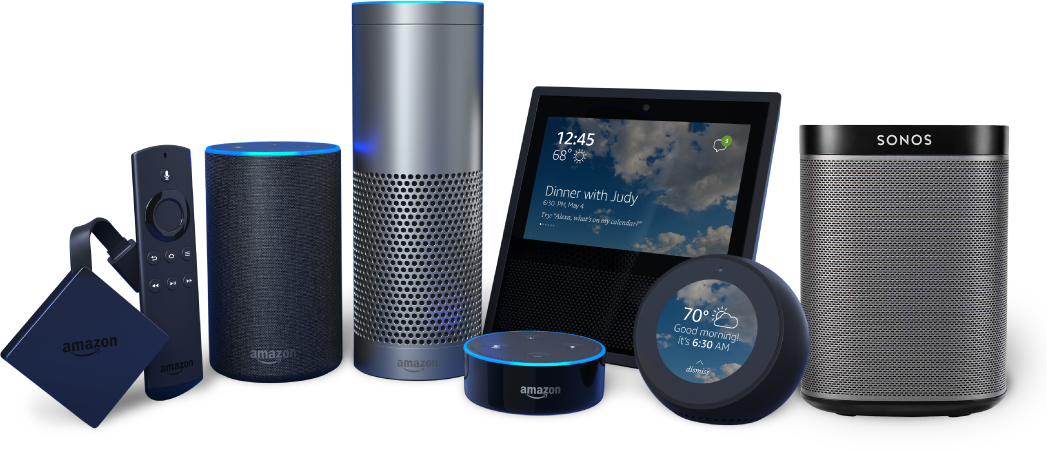
\includegraphics[scale=.8]{alexa_devices}
	\caption*{\footnotesize{Quelle: \mycite{figure_alexa_devices}}}
	\label{fig:alexa_devices}
\end{figure}

Unter \ac{ASR} versteht man die Umwandlung von menschlicher Sprache in Text.
Die Auslagerung der Rechenleistung in die Cloud sorgt für eine Beschleunigung der \ac{ASR}, sodass nahezu keine Latenz zu bemerken ist.\myfootcite[Vgl.][]{alexa_asr}

Lokal ist eine weitere \ac{ASR} Einheit verbaut, welche im Betrieb nach dem Stichwort \glqq Alexa\grqq \ lauscht.
Bei Erkennung des Stichworts werden nachfolgende Spracheingaben in Echtzeit an die Amazon Cloud gesendet.
Dort wird zunächst durch \ac{ASR} die Spracheingabe in Text konvertiert.
Anschließend wird durch \ac{NLU} über Mustererkennung die Bedeutung der Worte identifiziert. \myfootcite[Vgl.][]{alexa_nlu}

So können Befehle an ein Alexa Gerät weitergeben werden, welche über \ac{AWS}, Amazons Cloud, mit beliebigen Aktion verknüpft werden können.
Bspw. kann der Befehl \glqq Alexa, mach mir einen Kaffee.\grqq \ über \ac{AWS} mit der \ac{IoT}-Steuerung einer Kaffeemaschine so verknüpft werden, dass diese dann einen Kaffee produziert.
Die Verknüpfung von Befehl und Aktion über Alexa wird als \glqq Alexa Skill\grqq bezeichnet.
Zusätzlich gibt es \glqq Alexa Routines\grqq, welche keine Benutzereingaben entgegennehmen, also Automatisierungen darstellen können.

Mit Alexa Skills und Routines können Steuerungsebene, aber auch Automatisierungsebene eines Smart Home Systems realisiert werden.\myfootcite[Vgl.][]{alexa_skills_kit}

\begin{wrapfigure}{r}{0.35\textwidth}
	\centering
	\caption{Works with Alexa Siegel}
	
\includegraphics[scale=.5]{works-with-alexa}
	\caption*{\footnotesize{Quelle: \mycite{figure_works_with_alexa}}}
	\label{fig:works_with_alexa}
\end{wrapfigure}

Smart Home Produkte werden über das Internet mit Alexa verbunden.
Über Skills oder manuelle Programmierung kann ein Gerät, sofern es über ein öffentliches \ac{API} verfügt, angebunden werden.
Um diesen Prozess noch weiter zu vereinfachen können Hersteller die Zertifizierung \glqq Works with Alexa\grqq \ für ihre Produkte erlangen, wenn Spezifikationen bzgl. Installation des Produkts, sowie dessen Schnittstelle erfüllt werden.
\autoref{fig:works_with_alexa} zeigt das Works with Alexa Siegel, welches bei erfolgreicher Zertifizierung benutzt werden darf.
Für Besitzer von zertifizierten Geräten gibt es meist nur noch ein kurzen standardisierten Einrichtungsprozess zu überwinden.\myfootcite[Vgl.][]{workswithalexa}

\subsubsection{Vorteile}

Amazon Alexa zeichnet sich primär durch die einfache Handhabung aus.
Für die Nutzung und Einrichtung eines Amazon Alexa Systems sind lediglich technische Grundverständnisse bzgl. Smartphones und Computer notwendig.
Dies wird vorallem durch ansprechende Benutzeroberflächen, die direkte sprachliche Kommunikation und zertifizierten Smart Home Produkten ermöglicht.
Auch die Anschaffung eines Alexa Systems ist durch Amazons E-Commerce Plattform einfach.

\subsubsection{Nachteile}

Aufgrund der zentralen Architektur des Amazon Alexa Systems ergeben sich jedoch auch Probleme.
Wird etwa die Verbindung zum Internet, miteinhergehend die Verbindung zu Amazons Rechenzentrum, unterbrochen kann das Smart Home nicht mehr gesteuert werden, Automatisierungen fallen aus und selbst die Verbindung der einzelnen Smart Home Produkte untereinander sind nicht mehr vorhanden.
Ebenso werden sämtliche Daten durch \ac{AWS} geleitet und nicht lokal gespeichert.
So setzt man die eigenen Daten dem Internet aus.
Ein lokales Speichern und Verarbeiten würde einem Angreifer zunächst die Herausforderung stellen das lokale Heimnetzwerk zu penetrieren.
Dazu wird der Quelltext von Amazon Alexa nicht veröffentlicht und es kann somit nicht nachvollzogen werden, wie die eigenen Daten verarbeitet werden und welche Sicherheitslücken evtl. bestehen.

\subsection{Home Assistant}

Home Assistant ist eine Open-Source-Software für Heimautomatisierung.
Durch den modularen Aufbau der Software können Entwickler einfach neue Smart Home Produkte implementieren.
So sind aktuell 1187 Smart Home Produkte über 46 Kategorien mit Home Assistant nutzbar.\myfootcite[Vgl.][]{hass_components}

\begin{figure}[ht]
	\centering
	\caption{Home Assistant Core Architektur}
	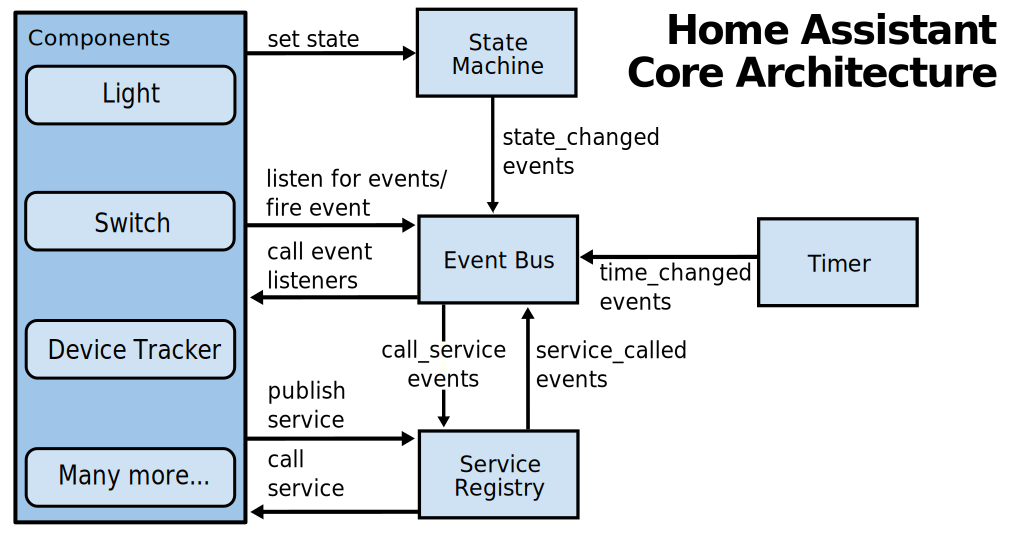
\includegraphics[width=0.9\textwidth]{hass_architecture}
	\caption*{\footnotesize{Quelle: \mycite{hass_architecture_figure}}}
	\label{fig:hasscorearch}
\end{figure}

\autoref{fig:hasscorearch} zeigt die Architektur, welche Home Assistant die Modularität verleiht.
Smart Home Produkte werden als Komponenten implementiert, welche mit dem Home Assistant Core interagieren.
Der Home Assistant Core besteht aus vier Modulen:

Das State Machine Modul bildet den Status der verschiedenen Komponenten ab.
Bemerkt ein Fenstersensor z.B. dass ein Fenster geöffnet wurde, aktualisiert die Komponente \textit{Fenstersensor} ihren Status im State Machine Modul, indem sie eine Nachricht an das Modul schickt.

Für zeitbasierende Automatisierungen existiert das Modul Timer, welches sekündlich ein Event emittiert.
Ein Event ist eine Nachricht, welche beim Auftreten von definierten Bedingungen automatsich verschickt wird.

Über das Event Bus Modul werden Events von den beiden bereits genannten Modulen empfangen von diesen ausgehend wiederum Events ausgelöst.

Das Service Registry Modul bietet Komponenten die Möglichkeit beim Gesamtsystem einen Service zu registrieren.
Das Gesamtsystem wiederum kann über das selbe Modul den Service einer Komponente in Anspruch nehmen.
So kann eine Glühbirne z.B. den Service \textit{Glühbirne anschalten} registrieren, welcher dann von einer anderen Komponente, z.B. einem Lichtschalter, indirekt, über ein Event, aufgerufen werden kann.

Mit dieser Architektur kann eine neue Komponente implementiert werden, ohne dass der Home Assistant Core berührt wird.
Eine neue Komponente muss lediglich einen Service registrieren, auf ein Event reagieren oder ein Event auslösen können.\myfootcite[Vgl.][]{hass_architecture}
Die Implementierung einer neuen Komponente ist ausführlich in der Home Assistant Dokumentation beschrieben.\myfootcite[Vgl.][]{hass_implement_component}

Veröffentlicht wird Home Assistant unter der Apache 2.0 Lizenz.\myfootcite[Vgl.][]{hass_license}
Die Software ist also kommerziell und privat kostenlos nutzbar.
Lediglich die Marke Home Assistant wird geschützt, sowie die Haftung und die Garantie ausgeschlossen.

Für die Weiterentwicklung von Home Assistant wurden im September 2018 vier Grundsätze definiert\myfootcite[Vgl.][]{hass_vision}:

\begin{itemize}
	\item Privatsphäre - alle Daten werden lokal verarbeitet und gespeichert.
	\item Lokale Kontrolle - es ist kein Internetanschluss notwendig.
	\item Offener Quelltext - die Funktionsweise kann jederzeit nachvollzogen werden.
	\item Interoperabilität - es soll einfach sein Apps mit Home Assistant zu verbinden
\end{itemize}

Ebenso wurde Nabu Casa Inc., als Modell für die Finanzierung der Entwicklung von Home Assistant, vorgestellt.
Home Assistant Nutzer können ihre private Instanz mit Nabu Casa um die Home Assistant Cloud Komponente für 5 USD pro Monat erweitern, was Home Assistant \ac{IoT}-Charakter verleiht.
Nabu Casa setzt dazu Software mit offenem Quelltext ein, verspricht keine Daten zu speichern und stellt dem Projekt Home Assistant Entwicklungkapazitäten zur Verfügung.\myfootcite[Vgl.][]{nabucasa}

\subsubsection{Vorteile}

Mit Home Assistant lassen sich hohe Kosten für zertifizierte Geräte sparen.
Während andere Smart Home System Anbieter, wie z.B. Amazon Alexa, Geräteherstellern die Implementierung von geeigneten Schnittstellen vorschreiben, damit die Geräte mit der jeweiligen Plattform genutzt werden können\myfootcite[Vgl.][]{workswithalexa}, bietet Home Assistant viele verschiedene Wege ein Geräte zu verbinden.
So sind über 1000 Schnittstellen bereits in Home Assistant implementiert\myfootcite[Vgl.][]{hass_components} und zusätzlich können neue oder eigen gebaute Geräte mit neuen Schnittstellen mit etwas Programmierkenntnissen selbst implementiert werden.\myfootcite[Vgl.][]{hass_implement_component}

\begin{wrapfigure}{r}{0.4\textwidth}
	\centering
	\caption{ESP8266 Board}
	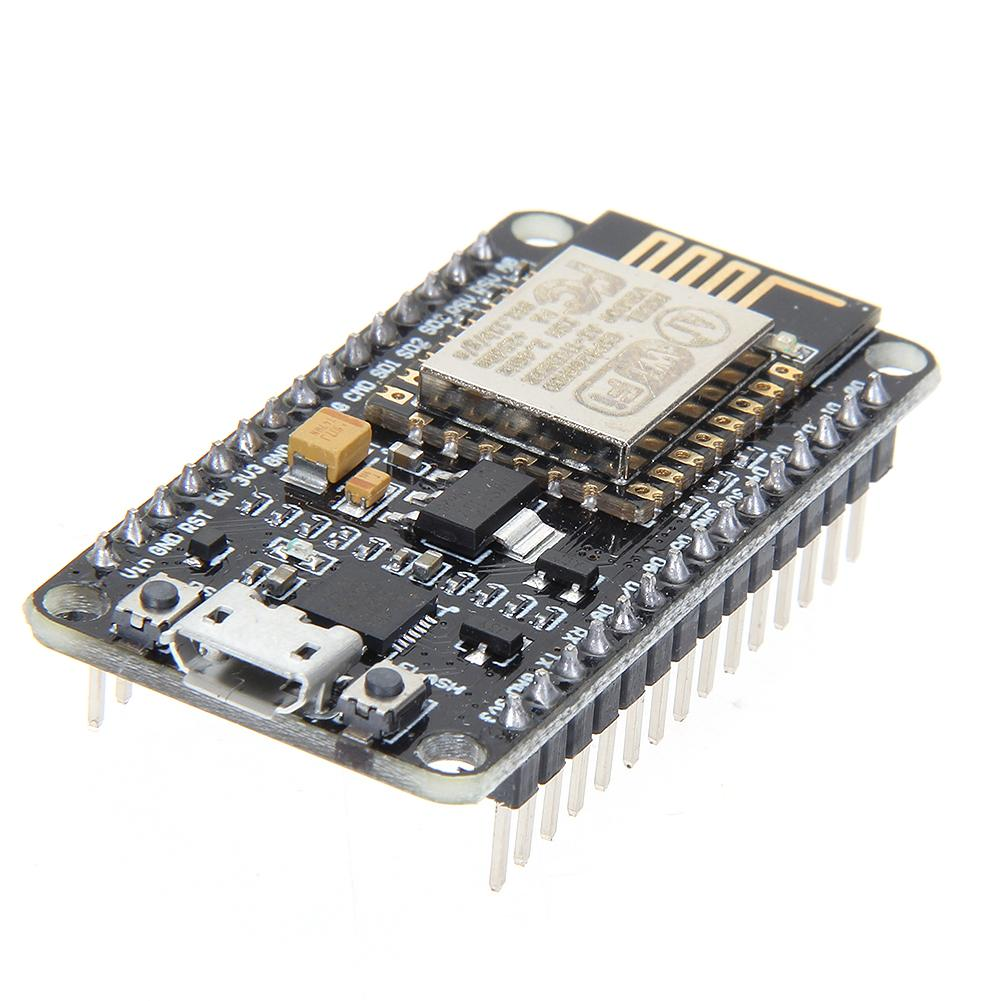
\includegraphics[scale=.1]{esp8266}
	\caption*{\footnotesize{Quelle: \mycite{esp8266}}}
	\label{fig:esp8266}
\end{wrapfigure}

\autoref{fig:esp8266} zeigt einen ESP8266 WLAN Mikrocomputer.
In Kombination mit einem Netzteil und Sensoren für Temperatur, Licht und Bewegung kann so eine \ac{DIY}-Wetterstation für weniger als zehn Euro gebaut werden.\myfootcite[Vgl.][]{bruhautomation_esp_sensor}

Der offene Quelltext von Home Assistant ermöglicht zudem, dass jederzeit nachvollzogen werden kann, was mit den eigenen Daten passiert.
Außerdem funktioniert Home Assistant vollständig offline.
Bei einem Internetausfall bleibt das Smart Home also weiter nutzbar.
Gleichzeitig bedeutet das auch, dass Dritte sich erst Zugriff zum eigenen Heimnetzwerk verschaffen müssen, damit ein Versuch unternommen werden kann Daten zu kompromittieren.

Zusammenfassend bietet Home Assistant Privatsphäre, Unabhängigkeit gegenüber des Internets, sowie eine hohe Bandbreite an verfügbaren Geräten und nutzbaren Schnittstellen.

\subsubsection{Nachteile}

Home Assistant wird von einer \glqq worldwide community of tinkerers and DIY enthusiasts.\grqq{}\myfootcite{hass_github_organization} entwickelt.
Gleichermaßen richtet sich Home Assistant als Produkt auch an Bastler und Tüftler.
So müssen Englischkenntnisse und Erfahrung im Umgang mit Linux und Computernetzwerken für die Einrichtung von Home Assistant vorhanden sein.\myfootcite[Vgl.][]{hass_getting_started}

Zudem befindet sich Home Assistant noch in aktiver Entwicklung und so fordern manche Änderungen der Software aktive Maßnahmen des Benutzers, wie etwa das Aktualisieren einer Konfigurationsdatei.\myfootcite[Vgl.][]{hass_breaking_change_example}

Home Assistant kann im jetzigen Zustand nur von technisch Versierten genutzt werden.

\subsection{\textbf{TODO} Integrierte Lösung} % change title to actual product

% ein system, welches beim bau eines haus integriert wird.
% also ein gesamtsystem aus einer hand von einem unternehmen.

\subsubsection{\textbf{TODO} Vorteile}

\subsubsection{\textbf{TODO} Nachteile}

\subsection{\textbf{TODO} Risiken}

% if used in combination with IoT: data breaches and loss of control
% power loss = no function
% smart home device with security flaw can be used to break into the local network

\subsection{\textbf{TODO} Geschäftsmodelle}

% foreach:
% how does the business model work?
% example product?
% potential market?

\subsubsection{\textbf{TODO} Geräte verkaufen} % TODO better title

% sell products like: philips lightning bulb

\subsubsection{\textbf{TODO} Cloud Erweiterung} % TODO better title

% see: home assistant cloud by nabu casa

\subsubsection{\textbf{TODO} Gesamtsystem} % TODO better title

% install a smart home integration in peoples homes who don't know how to do so themselves

\subsubsection{\textbf{TODO} Alexa Skills} % TODO better title

% sell alexa skills
% create a skill with payment option

% https://developer.amazon.com/blogs/alexa/post/b8101123-f1b9-494c-8bbb-53e3850a1123/in-skill-purchasing-offers-jeff-bolton-s-voice-business-a-new-level-of-monetization

\section{\textbf{TODO} Fazit}

% trends --> closed source, iot :/, automations! :D
% best business models
% home assistant empfehlung :)